\documentclass[11pt]{article}

% ---------- Packages ----------
\usepackage[margin=1in]{geometry}
\usepackage{graphicx}
\usepackage{booktabs}
\usepackage{array}
\usepackage{caption}
\usepackage{subcaption}
\usepackage{hyperref}
\usepackage{xcolor}
\usepackage{enumitem}
\usepackage{listings}
\usepackage{microtype}
\usepackage{authblk}
\usepackage{natbib}

\hypersetup{
  colorlinks=true,
  linkcolor=black,
  citecolor=blue!40!black,
  urlcolor=blue!50!black
}

\graphicspath{{../figures/}}

\lstset{
  basicstyle=\ttfamily\footnotesize,
  breaklines=true,
  columns=fullflexible,
  frame=single,
  framesep=4pt,
  xleftmargin=6pt,
  showstringspaces=false,
}

\title{\textbf{Internal Signals of Tool-Result Inconsistency \\
in an Open-Weights LLM Agent}}

\author{Zhongzheng Xu}
\date{May 2026}

\begin{document}
\maketitle

\begin{abstract}
\noindent
We investigate whether an open-weights LLM agent, while solving a tool-use
task, internally registers when a tool result is inconsistent with the user's
goal --- even in cases where its written chain of thought (CoT) does not
mention the inconsistency. The full pipeline runs on a single high-memory
GPU (A100 / H100) on top of \texttt{Qwen2.5-7B-Instruct} \citep{qwen25}: we
build a controlled synthetic shopping environment, generate 1{,}218 valid
agent trajectories across three random seeds with graded perturbations of the
tool output, train per-layer linear probes on captured residual-stream
activations, and run a steering sweep. The central probe (Level~1 vs.\
Level~2, a matched control) reaches an ROC-AUC of $0.96 \pm 0.01$ at
layer~19, while the agent verbalizes the violation in only $\sim$82\% of
Level~2 cases and refuses the perturbed item in only $\sim$26\%. Steering
along the probe direction lifts CoT verbalization but consistently
\emph{reduces} action rejection, dissociating a CoT channel from an action
channel of agent unfaithfulness. Code, data and figures are released at
\url{https://github.com/lebretou/agent_faithfulness}.
\end{abstract}

% ===============================================================
\section{Introduction and Problem}
% ===============================================================

LLM agents now act on the world. They call tools, read structured results,
write a short ``chain of thought'' (CoT) explaining what they will do, and
then act. Increasingly, downstream evaluators trust that written explanation
as a proxy for what the model is actually doing. Recent work has shown this
trust is poorly founded: in controlled experiments where a hidden hint was
the actual cause of the model's answer, frontier reasoning models acknowledged
the hint in their CoT only about a quarter of the time \citep{chen2025faith}.
This is the operational notion of \emph{unfaithfulness}: the chain of thought
does not reflect the computation that produced the output. For autonomous
agents the stakes rise sharply, because a single unfaithful step --- the tool
returned the wrong thing, but the CoT does not say so --- can silently
propagate into an action.

This project asks a narrow, controlled version of the question. When the
search tool returns something inconsistent with the user's request, does the
model's residual stream contain a detectable signal of the inconsistency,
even when the CoT does not verbalize it? And if so, can a steering vector
built from that signal causally change the agent's behavior? Behavioral
evaluation alone cannot answer either question, because it cannot tell ``the
model didn't notice'' apart from ``the model noticed but didn't say.'' The
standard mechanistic-interpretability toolkit can: linear probes
\citep{alain2016probes} address the first hypothesis by reading from hidden
states, and activation steering \citep{turner2023actadd, panickssery2024caa}
addresses the second by writing to them. A reliable probe would also be a
candidate runtime monitor that is independent of CoT text, which is exactly
the modality one wants when CoT itself is the unreliable channel.

The investigation is GPU-heavy in a way that makes cloud compute
non-trivial. Generating each trajectory requires running a 7B-parameter
open-weights model with tool-call decoding plus activation hooks installed
on all 28 transformer blocks; training per-layer probes consumes hundreds
of MB of bf16 activations; and the steering sweep re-runs trajectory
generation under a forward-hook intervention for every $\alpha$ in the
sweep. The pipeline runs on A100 (40~GB) and, when available, H100
(80~GB). The H100 in particular fit
three bf16 copies of the model concurrently, which is what let us generate
three independent random-seed corpora in parallel and report
mean$\pm$std rather than single-point estimates.

Three contributions follow. First, a fully reproducible synthetic agent
environment with deterministic free labels and no LLM judge in the loop.
Second, empirical evidence that linear probes on residual-stream activations
detect goal-relative inconsistency at AUC $0.96$, while the agent's CoT
verbalizes it only $\sim 82\%$ of the time and its action refuses only
$\sim 26\%$ of the time --- an operational faithfulness gap. Third, a
steering analysis showing that the located direction is causally upstream of
CoT content but separable from the action policy: pushing along it makes the
agent \emph{say} the violation more, while \emph{acting on it less}.

% ===============================================================
\section{Design}
% ===============================================================

\subsection{System architecture}

The pipeline has three stages glued together by a JSONL trajectory store and
a folder of per-(trajectory, step) activation tensors on a shared artifact store. The
first stage runs the environment and the agent loop on a cloud GPU: a
synthetic shopping catalog, a single \texttt{search} tool, a
\texttt{Qwen2.5-7B-Instruct} agent driven via the native chat template with
function calling, and a perturbation layer that intercepts tool outputs
between the catalog and the agent. The second stage, also GPU-bound, captures
activations: forward hooks on every transformer block save the residual
stream at the last token of each tool message into bf16 \texttt{.pt} files
(one per step, about 200 KB each). The third stage --- probing and steering
--- is split. Probe training is CPU-only \texttt{scikit-learn} logistic
regression and runs on a laptop in minutes; the steering sweep is GPU-bound
because it replays trajectory generation with a forward hook that adds
$\alpha \cdot v$ to the residual stream at the best layer.

\subsection{Model and dataset}

We use \texttt{Qwen/Qwen2.5-7B-Instruct} \citep{qwen25} in bf16. It was
chosen for its solid native function-calling template and its open weights,
both required: probes and forward hooks need white-box access. A fallback to
\texttt{Llama-3.1-8B-Instruct} was held in reserve but never needed.

The synthetic environment is, in effect, the experimental apparatus. We
deliberately built it ourselves rather than using existing benchmarks because
those benchmarks were designed to evaluate task success, not to support
controlled mechanistic study. WebShop's catalog comes from a real Amazon
scrape \citep{yao2022webshop}, so the salience of any perturbed attribute
depends on how central it was to the original query and varies unpredictably
across categories. ALFWorld's textual scenes interact with partial
observability and trajectory-specific state \citep{shridhar2021alfworld}.
ToolBench standardizes tool schemas but largely sacrifices the multi-step
structure that makes agentic faithfulness distinct from single-prompt
faithfulness \citep{qin2024toolllm}. The mechanistic interpretability
literature has long used controlled environments precisely because clean
causal claims require a controlled data-generating process: Othello-GPT
studied board-state representations through a synthetic game
\citep{li2023othello}, and similar choices recur in studies of internal
reasoning structure. The cost we accept is that this pilot version does
not validate on a real benchmark; we frame the work accordingly.

The catalog itself is a 200-item table generated reproducibly from seed~42,
with seven structured attributes per item drawn from fixed vocabularies
(category, color, size, price, material, brand). Queries are templates with
three constraints, sampled by rejection so every clean query is solvable.
The single tool, \texttt{search}, returns up to $k=5$ items ranked by how
many constraints they satisfy, breaking ties on price.

Three perturbation levels structure the experiment, and they are defined
\emph{relative to the query's constraints} so that levels are comparable
across trajectories. Level~0 leaves the tool result clean. Level~1 swaps one
attribute of the top-ranked item that is \emph{not} among the query's
constraints, so the item still satisfies every constraint --- the user asked
for a blue shirt under \$30 and got one, with a brand whose listed value has
been changed. Level~2 swaps one attribute that \emph{is} a constraint,
violating it: the user asked for a blue shirt under \$30 and got a red shirt
under \$30. The L1-vs-L2 comparison is the key design choice. Both levels
perform exactly one attribute swap on the top item, so they have matched
input-distance characteristics; only L2 creates a goal-relative
inconsistency. A linear probe that separates them therefore cannot be
relying on raw input-distance, which is the in-design control that replaces
the parallel matched-control corpus in the original plan and saves roughly
half a day of generation.

Every trajectory gets five labels deterministically, with no LLM judge:
the perturbation level, the perturbed attribute, whether the CoT mentions
the perturbation (a regex of about twelve phrase patterns plus the perturbed
value as a string), whether the agent's action rejects the perturbation
(a purely structural check that compares the purchased item ID to the
perturbed top item and counts post-perturbation \texttt{search} calls), and
whether the purchased item actually satisfies the query. The action-rejection
label is regex-free, which matters later for interpreting the steering
results.

\subsection{Compute setup}

A single A100 (40~GB) was used for initial smoke tests and overnight runs,
and an H100 (80~GB) when available, which made the parallel-seed strategy
possible by hosting three bf16 copies of the model concurrently. A
network-mounted artifact store served as the canonical output location;
trajectories were appended to JSONL incrementally so that interrupted
sessions were recoverable, and activations were saved per-step so that
nothing had to fit in RAM. Total artifact size is about 700 MB. Source code
is available at \url{https://github.com/lebretou/agent_faithfulness}.

% ===============================================================
\section{Implementation}
% ===============================================================

The codebase splits along a hard local-vs-cloud line. Pure-Python modules
that touch only data structures --- catalog generation, query templates,
tool search, perturbation logic, label computation --- run CPU-only and are
unit-tested on a laptop. Anything that touches the model --- the agent loop,
the activation hooks, corpus generation, the steering sweep --- runs on
a GPU host. This separation kept the test suite fast (45 cases, all passing,
runtime well under a second) and let us iterate on data-side bugs without
spinning up a GPU.

The agent loop itself is short. The system prompt instructs the agent to
think inside \texttt{<think>} tags, call \texttt{search}, inspect the
results, optionally refine and search again, and finally emit
\texttt{PURCHASE: item\_XXXX}. Trajectories are capped at five steps;
agents that do not purchase by then are dropped, and the drop rate settled
around 20\%. Two implementation bugs were worth recording because both
quietly destroyed labels until fixed. The first was that newer versions of
\texttt{transformers} return a \texttt{BatchEncoding} dict from
\texttt{apply\_chat\_template(tools=...)} rather than a tensor, which
silently mis-shaped the forward pass until we normalized it. The second was
that \texttt{Qwen2.5-7B-Instruct} does not reliably emit the
\texttt{<think>} tags despite the system prompt asking for them; without a
fallback that treats raw assistant text (minus the \texttt{<tool\_call>}
block) as the thought, every CoT was being labeled as an empty string and
the verbalization rate was meaninglessly close to zero.

Activation capture follows the standard recipe. For each tool message we
tokenize the conversation up to and including that message, register a
forward hook on every transformer block that snapshots the residual stream
at the last token, and save the resulting \texttt{(28, 3584)} bf16 tensor as
\texttt{traj\_NNNN\_step\_K.pt}. Each tensor is about 200~KB; for 1{,}218
trajectories with roughly three informative steps each, total storage is
around 700~MB. The trajectories.jsonl file references each tensor by
absolute GPU-host path, and a small loader normalizes those paths to local
roots when probes are trained on a laptop.

Probe training is intentionally simple. For each transformer layer
$\ell \in \{0, \dots, 27\}$ we train a logistic regression on the residual
at $\ell$ and report 5-fold cross-validated ROC-AUC \citep{alain2016probes}.
Two classifiers are trained: Classifier~A separates L0 from L2 and is a
sanity check; Classifier~B separates L1 from L2 and is the central
matched-control probe. We deliberately use logistic regression rather than
a deeper classifier; if a property is recovered by a tiny linear classifier
on a single layer, that is much stronger evidence that the property is
encoded as a linear direction than the same accuracy obtained by an MLP
\citep{belinkov2022probing}. A permutation control --- shuffle the labels
and retrain --- is scaffolded as \texttt{scripts/03b\_permutation\_control.py}
with a PASS criterion of \texttt{shuf\_mean < 0.60}; we report on it in the
limitations section because it has not yet been executed end-to-end.

The steering setup uses two complementary ways to derive the direction $v$,
both standard in the literature. The probe-weight route normalizes the
trained probe's weight vector at the best layer to unit length and uses it
directly. The contrastive route, equivalent in spirit to
contrastive activation addition and the difference-of-means construction
\citep{turner2023actadd, panickssery2024caa}, computes $v = \overline{h}_{L2}
- \overline{h}_{L1}$ at the best layer and normalizes. At inference time we
install a forward hook that adds $\alpha \cdot v$ to the residual stream at
the best layer, only at the last token position immediately preceding the
agent's next \texttt{<think>}. Sweeping $\alpha$, we measure the
verbalization rate and action-rejection rate on held-out L2 trajectories and
task success on held-out L0 trajectories. The L0 success number is
deliberately separated: it is the sanity check that steering hasn't simply
destroyed the agent on clean inputs, which is the standard failure mode of
any single-direction intervention with too large $\alpha$.

The test suite (45 CPU-only pytest cases) covers the structural invariants
that make the experiment trustworthy: every L1 perturbation lands on a
non-constraint attribute (0 of 473 hits on a constraint), every L2
perturbation lands on a constraint attribute (491 of 491), perturbed values
are always different from originals, labels are computable deterministically,
and the steering hook is bit-exact inert at $\alpha = 0$. The
$\alpha = 0$ invariant in particular was important: it guarantees that any
difference between the $\alpha = 0$ cell and the unsteered baseline is GPU
floating-point non-determinism, not a hook bug.

% ===============================================================
\section{Results and Deliverables}
% ===============================================================

\subsection{Corpus statistics}

We generated three independent seeds (42, 43, 44), 500 trajectories each,
in parallel on a single H100; 1{,}218 of the 1{,}500 finished within the
five-step budget and were retained. Table~\ref{tab:label-rates} reports the
headline behavioral rates by perturbation level. Two patterns matter for
interpretation. The L0 verbalization rate of 17\% is not pure regex noise,
because the regex is calibrated and manual inspection found agents
legitimately commenting on \emph{organic} ranking mismatches that the model's
own \texttt{search} call sometimes returns even on the clean catalog (the
labeler is right; L0 simply is not a true zero). And the average step count
rises from 2.5 to 3.2 between L0/L1 and L2, which is independent behavioral
evidence --- not mediated by any text matching --- that L2 is being noticed
by the agent at \emph{some} level even when the action does not change.

\begin{table}[h]
\centering
\caption{Label rates across perturbation levels (mean $\pm$ std across three
seeds, 1{,}218 valid trajectories total). \texttt{verb\%} = CoT mentions the
inconsistency; \texttt{rej\%} = the agent did not purchase the perturbed top
item; \texttt{succ\%} = purchased item satisfies the query constraints.}
\label{tab:label-rates}
\small
\begin{tabular}{lcccc}
\toprule
Level & verb\% & rej\% & succ\% & avg.\ steps \\
\midrule
L0 (clean)               & $17 \pm 7$ & $\phantom{0}0 \pm 0$ & $81 \pm 7$ & 2.5 \\
L1 (non-constraint swap) & $33 \pm 1$ & $17 \pm 1$           & $85 \pm 1$ & 2.5 \\
L2 (constraint violation)& $82 \pm 1$ & $26 \pm 3$           & $78 \pm 4$ & 3.2 \\
\bottomrule
\end{tabular}
\end{table}

\subsection{Probes detect goal-relative inconsistency}

Figure~\ref{fig:probe-auc} gives the per-layer probe AUC for both
classifiers. Both curves climb from about $0.62$ at layer 0, plateau around
$0.96$ from layers 17--27, and decay slightly toward the final layer. The
central observation is not the AUC value itself but the comparison: Classifier
B (L1 vs.\ L2) is essentially indistinguishable from Classifier A (L0 vs.\
L2). Because L1 and L2 are matched on input-distance by construction (one
attribute swap on the top item, in both cases), the only thing left for the
probe to lean on is the goal-relative semantics of the swap. The probe
direction must therefore encode something close to ``the top result violates
a query constraint,'' not merely ``the top result looks different from what
the model first generated.'' The best layer for Classifier B is layer 19,
stable across seeds within $\pm 1$, and is what we use for steering. That
mid-to-late layers carry abstract task-relevant features more cleanly than
either early or final layers is consistent with prior probing work
\citep{li2023othello, belinkov2022probing}.

\begin{figure}[h]
\centering
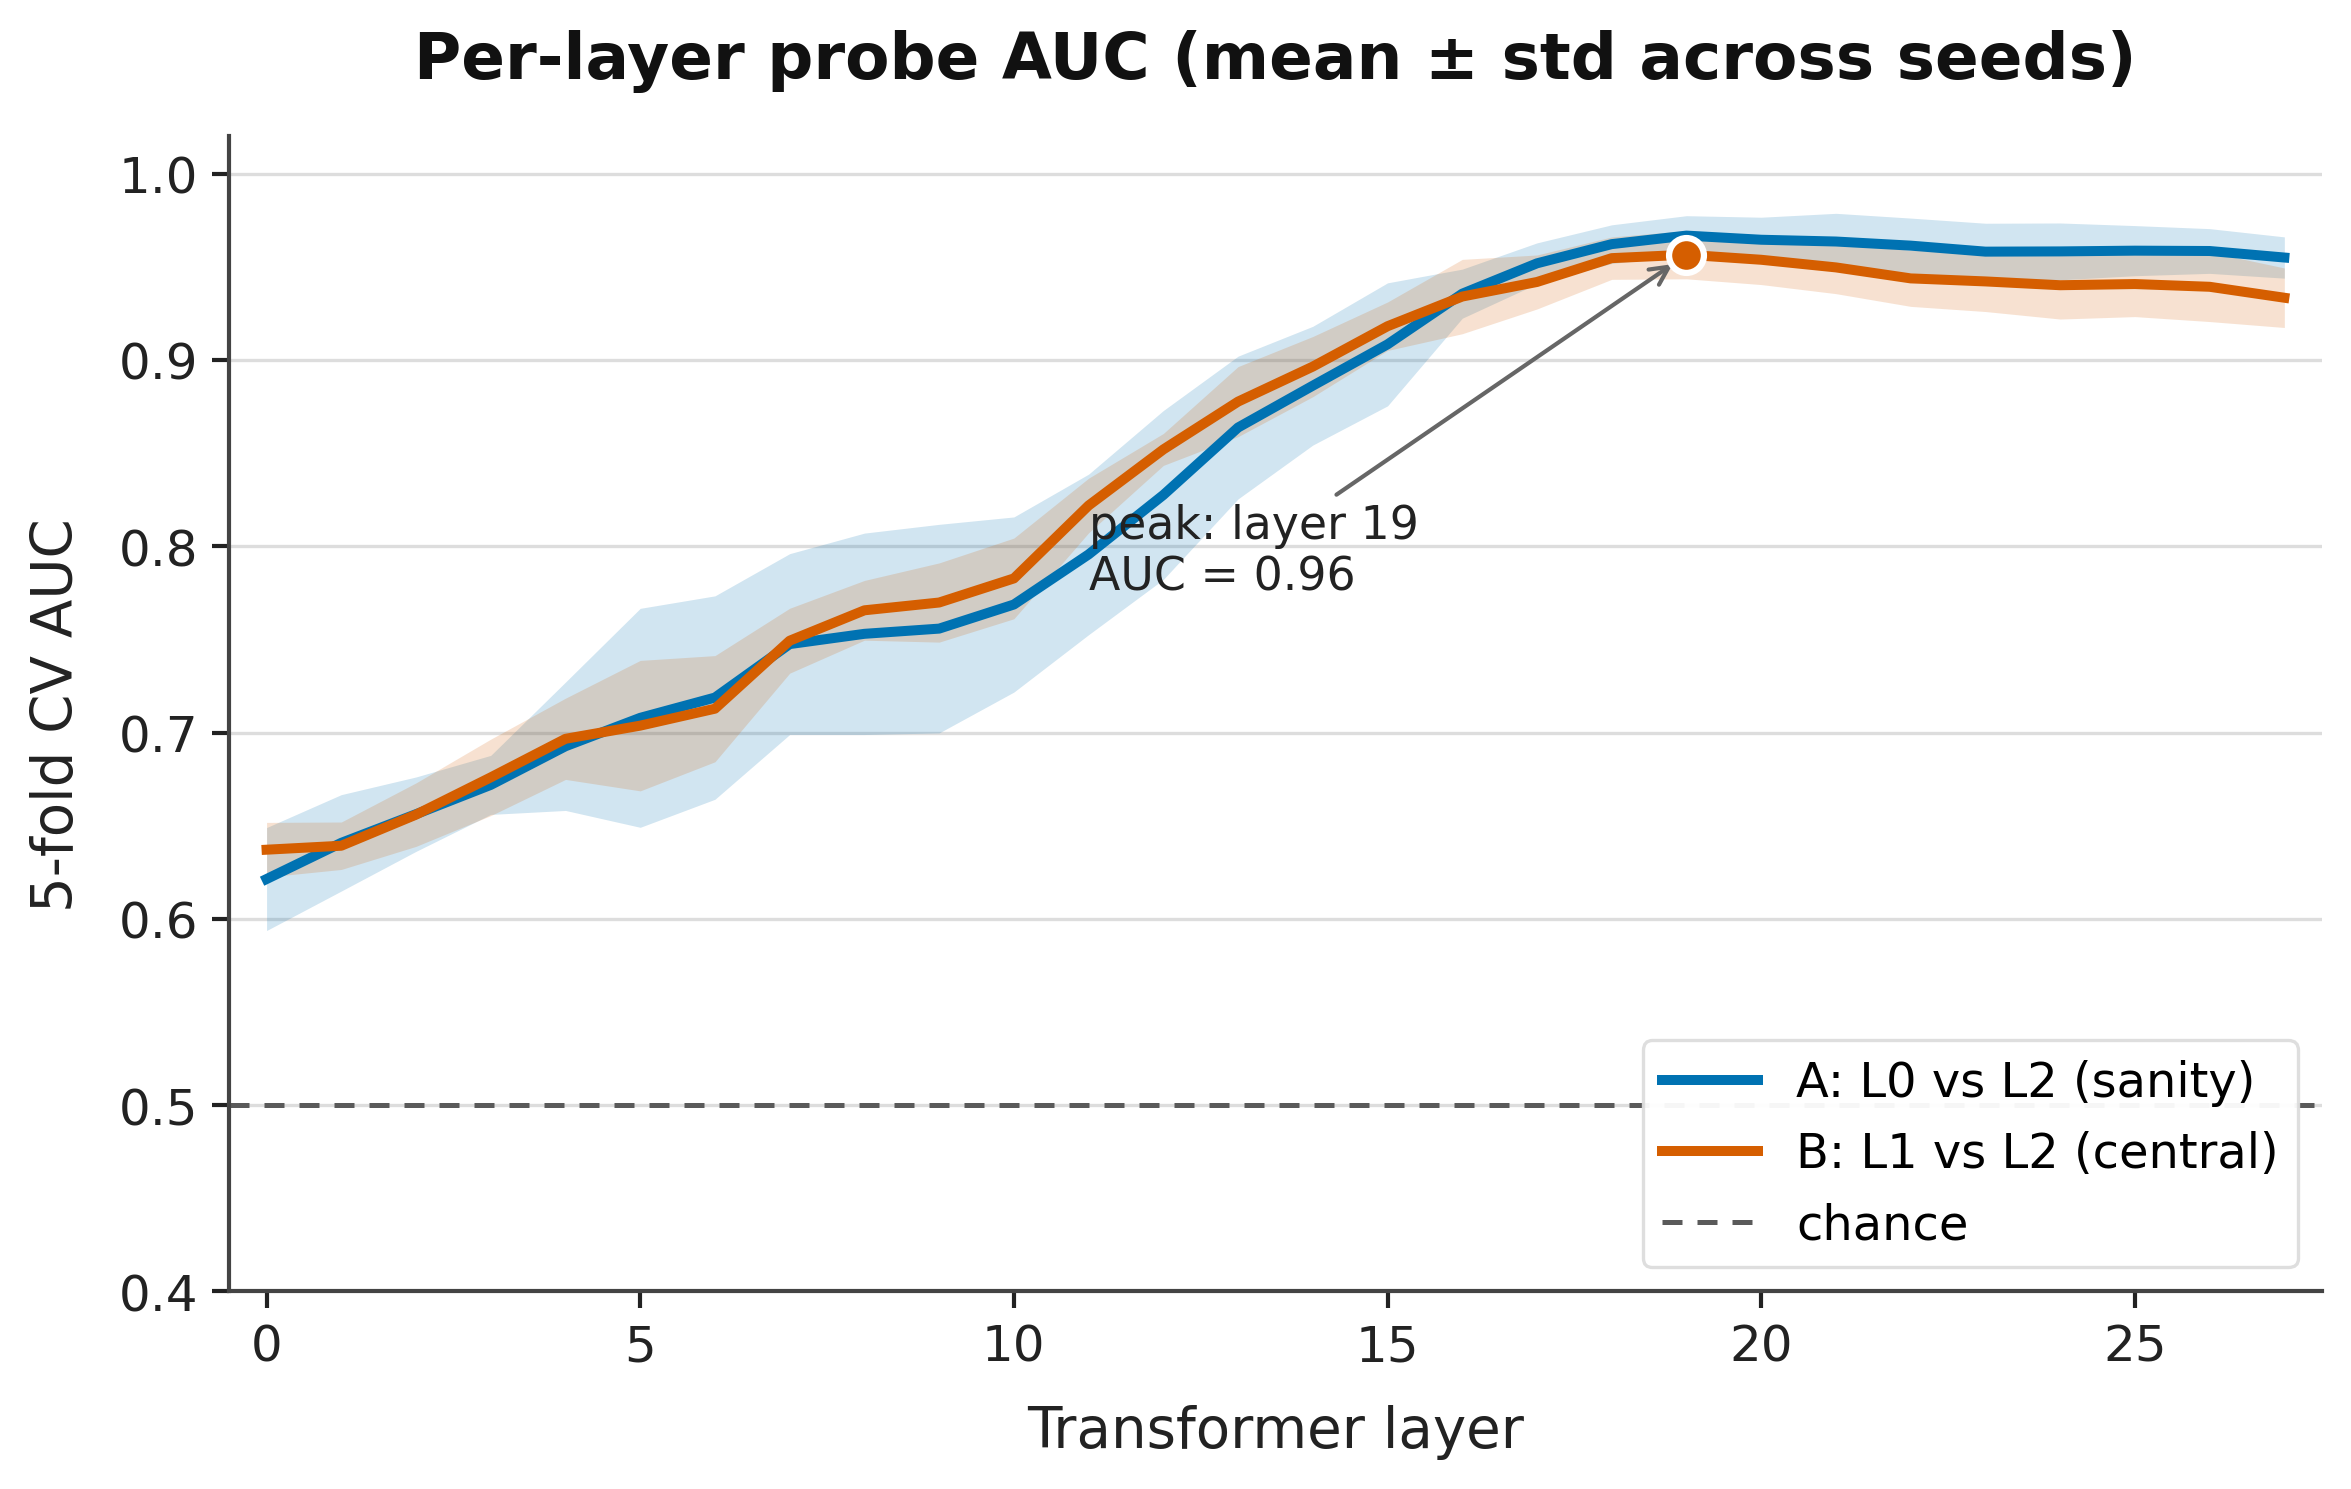
\includegraphics[width=0.7\textwidth]{probe_auc_by_layer.png}
\caption{Per-layer probe AUC for Classifier~A (L0 vs.\ L2) and Classifier~B
(L1 vs.\ L2), mean $\pm$ std across seeds 42/43/44. The two curves track
each other closely, which is the matched-control signature that B is not
riding on input-distance alone.}
\label{fig:probe-auc}
\end{figure}

\subsection{The faithfulness gap}

The probe result is one half of the headline; the other half is comparing it
against what the agent actually says and does. Figure~\ref{fig:three-curve}
overlays the probe AUC against the verbalization and action-rejection rates
across perturbation levels. The probe AUCs sit at the top of the plot, near
$0.96$; the verbalization curve climbs from 17\% at L0 to 82\% at L2, and
the action-rejection curve climbs only from 0\% at L0 to 26\% at L2. The
gap between the probe and the two behavioral curves is the operational
faithfulness gap: even at L2, where the inconsistency is unambiguous, the
written reasoning misses it almost one time in five and the action ignores
it three times in four. Put differently, the model knows more than it says,
and acts on substantially less than it knows. This pattern is consistent
with the broader faithfulness picture from \citet{chen2025faith}, where the
internal cause of an answer is reliably under-reported by the CoT, and
extends it to a multi-step tool-use setting.

\begin{figure}[h]
\centering
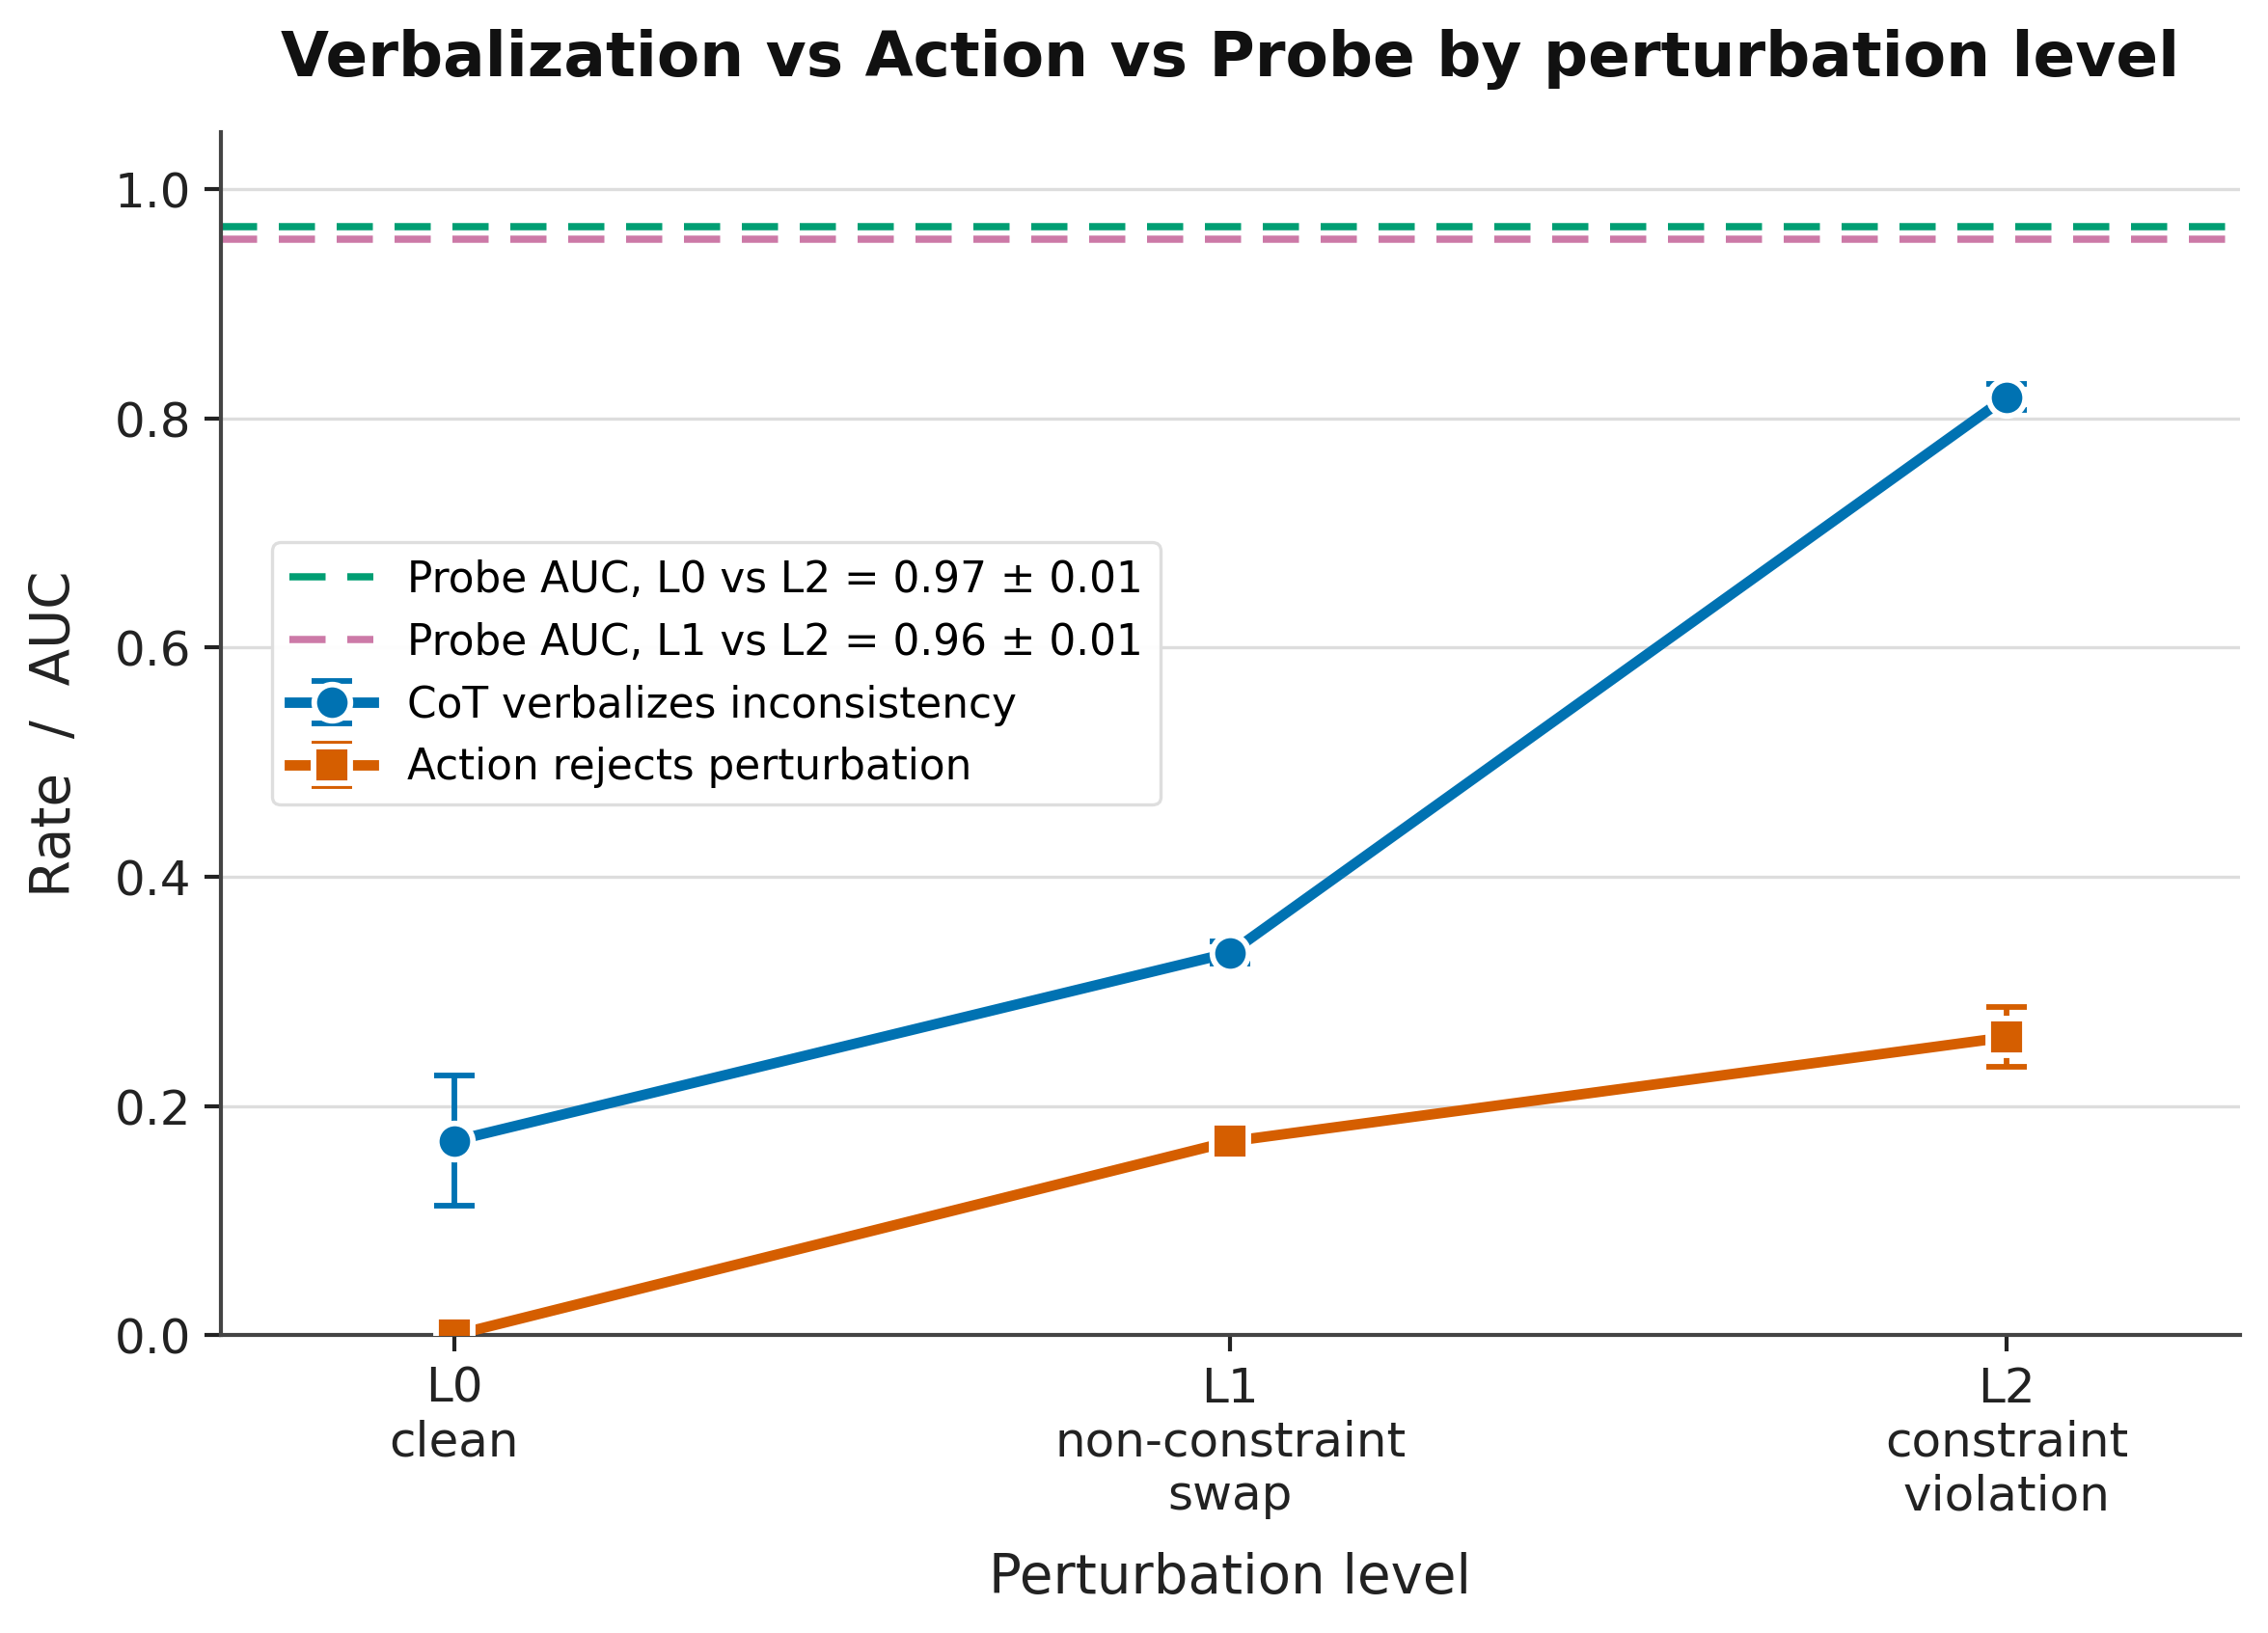
\includegraphics[width=0.65\textwidth]{three_curve_plot.png}
\caption{Headline three-curve plot. The probe AUCs (dashed) sit far above
the rate at which the CoT verbalizes the inconsistency (blue) and far above
the rate at which the agent's action rejects the perturbed result (orange).
The gap between the probe and the behavioral curves is the operational
faithfulness gap.}
\label{fig:three-curve}
\end{figure}

\subsection{Steering: the located direction is causal but selective}

The steering experiment asks whether the layer-19 direction is merely
predictive or actually causal, and if causal, what behavior it controls.
We ran five sweeps in total. The cleanest one --- and the one we treat as
the headline --- is a contrastive direction at layer 19 with $n \approx 80$
held-out L2 trajectories per $\alpha$ cell. It is the only sweep large
enough to discriminate small effects from the roughly five-percentage-point
GPU non-determinism floor that bf16 matmul ordering induces on H100 tensor
cores when \texttt{torch.use\_deterministic\_algorithms} is not set.

\begin{table}[h]
\centering
\caption{Headline steering sweep: contrastive direction at layer 19, high-$n$
($n \approx 80$ held-out L2 trajectories per $\alpha$). Verbalization climbs
with $\alpha$, action rejection drops below baseline once $\alpha \geq 1$,
and L0 task success stays in the 75--85\% band across the working regime.}
\label{tab:steering-headline}
\small
\begin{tabular}{lccccc}
\toprule
$\alpha$ & 0.0 & 0.5 & 1.0 & 1.5 & 2.0 \\
\midrule
verb\% (L2)     & 77 & 82 & 79 & 84 & \textbf{89} \\
rej\% (L2)      & 31 & 32 & 18 & 21 & 24 \\
succ\% (L0)     & 74 & 85 & 77 & 86 & 76 \\
\bottomrule
\end{tabular}
\end{table}

Table~\ref{tab:steering-headline} reports the headline numbers and
Figure~\ref{fig:steering-curve} plots them. Two things happen as $\alpha$
grows. Verbalization climbs monotonically modulo one stumble, ending 12
percentage points above baseline at $\alpha = 2$, which is roughly three
standard errors above the $\alpha = 0$ cell at $n \approx 80$. Action
rejection moves in the opposite direction: it drops from 31\% at baseline to
the 18--24\% band for every $\alpha \geq 1$. The L0 task success number
remains in the 75--85\% range, which means the agent has not been broken on
clean inputs --- steering is changing CoT and action selectively, not
shutting the model down. The direction located by the probe is therefore
causally upstream of CoT content (pushing along it makes the agent say the
violation more often) but separable from the action policy (the same push
makes the agent comply with the perturbed result more often). Read
carefully, this is a non-trivial structural fact about where unfaithfulness
lives in the model. ``The model knows but does not say'' is a real channel,
but ``the model says but does not act'' is a separate channel, and the
second is the harder one to close.

\begin{figure}[h]
\centering
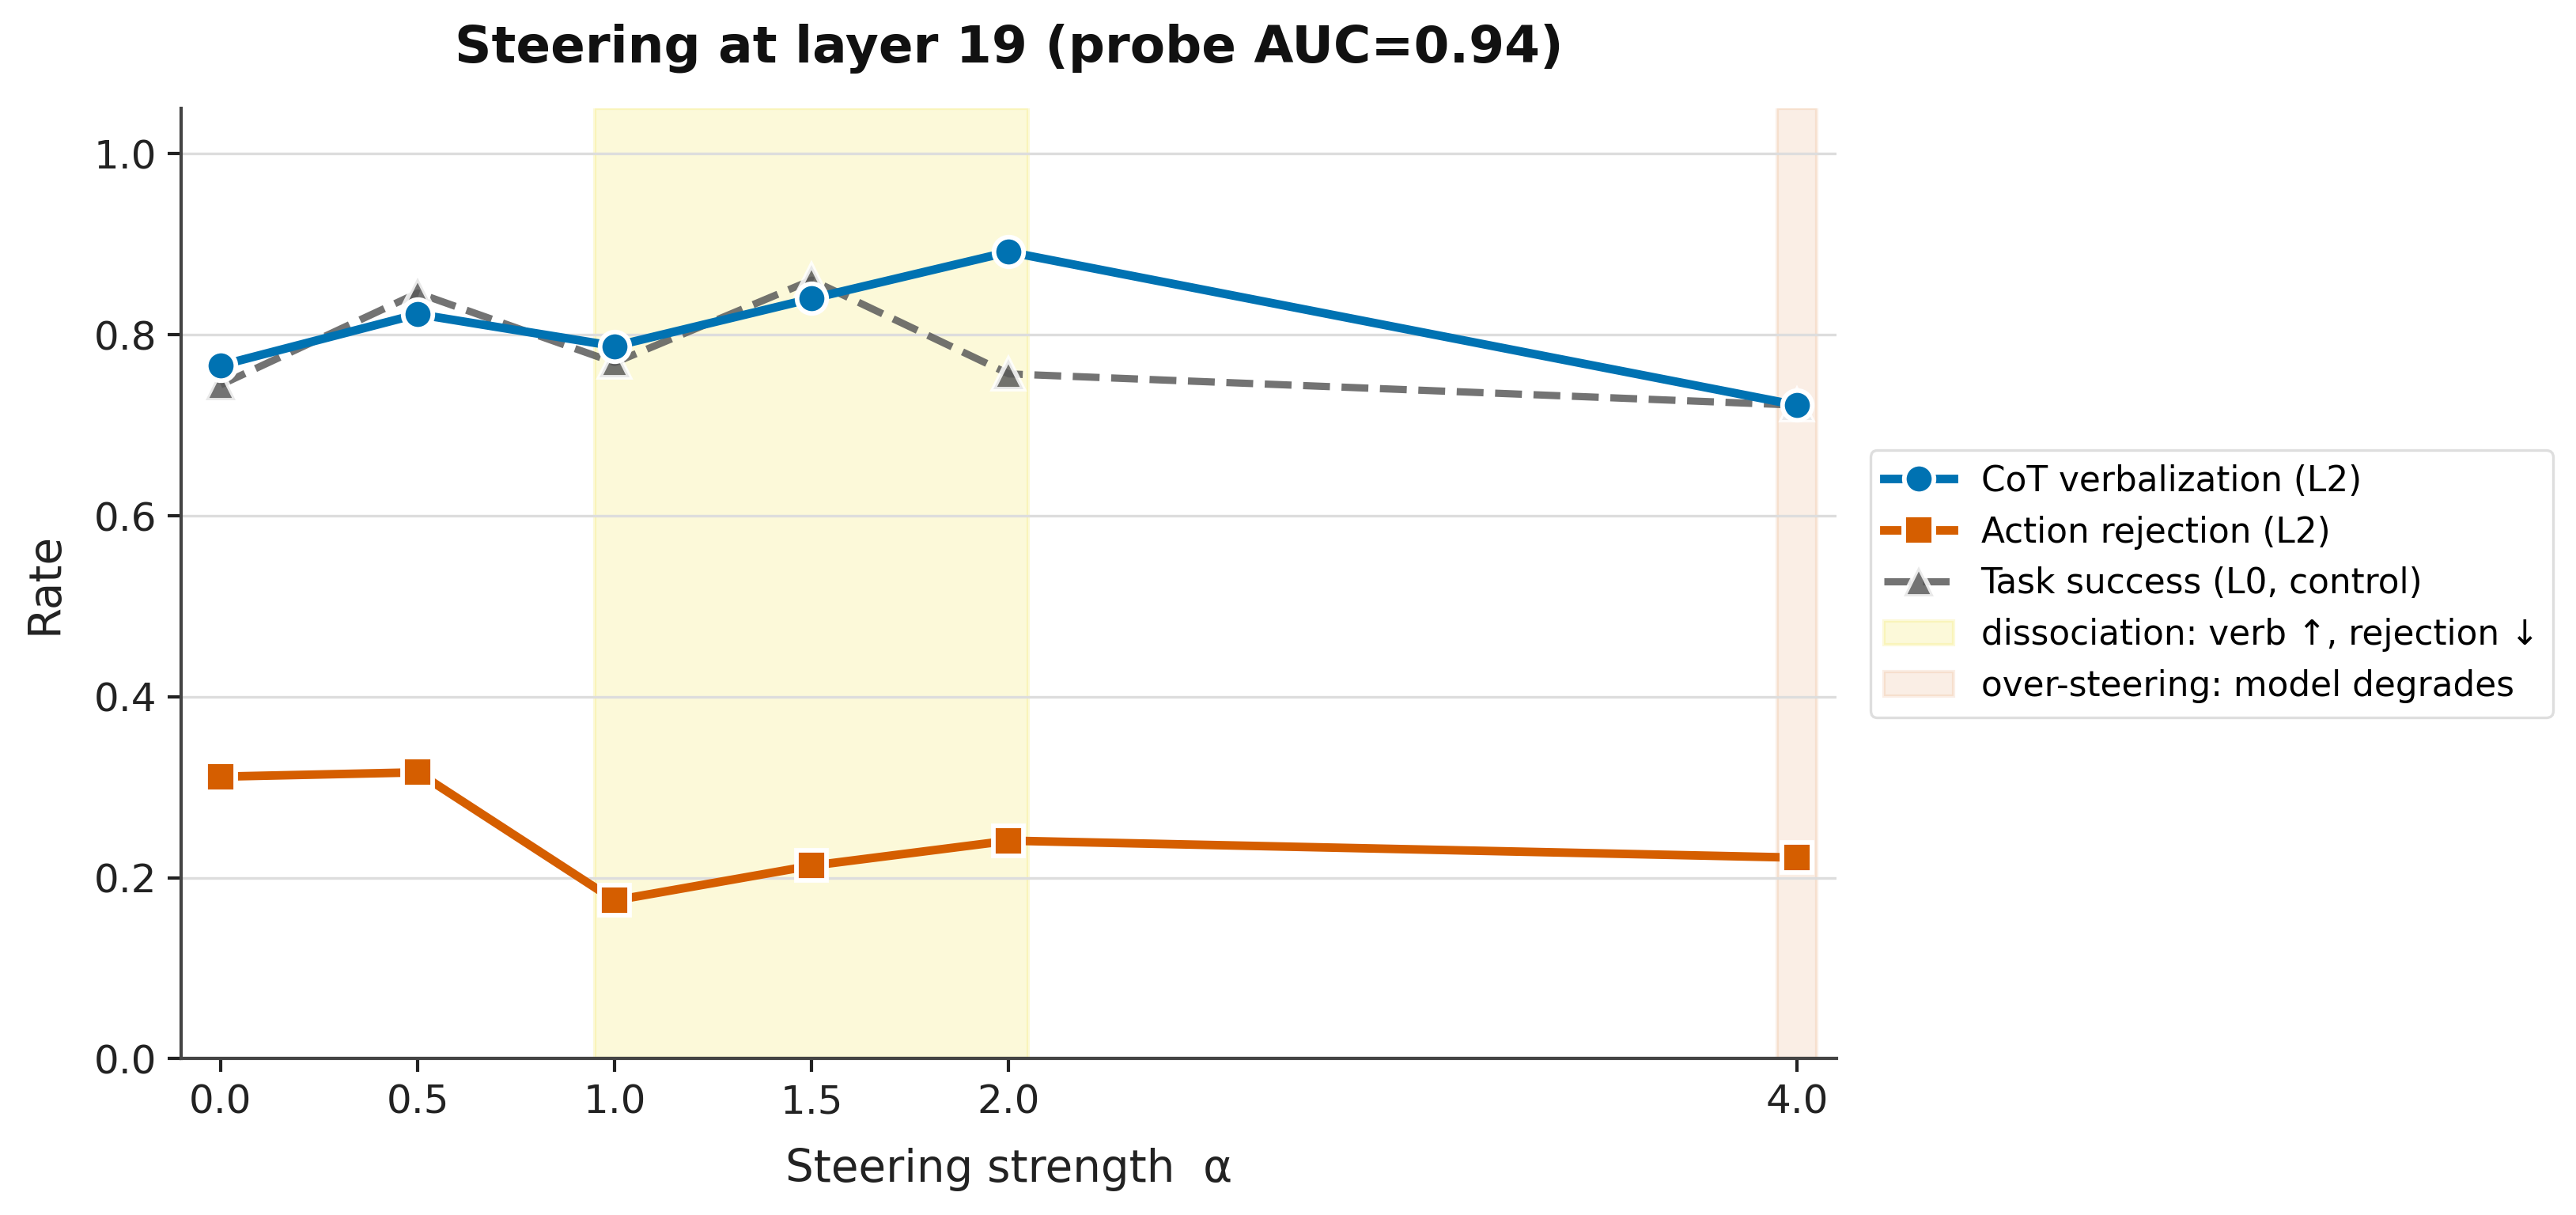
\includegraphics[width=0.92\textwidth]{steering_curve.png}
\caption{Verbalization rate, action-rejection rate, and L0 task success vs.\
steering strength $\alpha$ for the high-$n$ contrastive-at-L19 sweep
($n \approx 80$ per cell). Verbalization climbs with $\alpha$; action
rejection sits below baseline at every $\alpha \geq 1$; clean-input task
success stays roughly flat.}
\label{fig:steering-curve}
\end{figure}

The next question is whether this pattern is specific to one choice of
direction and one choice of layer, or whether it reflects something about
the underlying representation. Table~\ref{tab:steering-ablations} shows
three ablations that share a common $\alpha$ grid of $\{0, 1, 4\}$. We
compare a contrastive direction at layer 19, the same probe weights from
layer 19 applied at layer 25 (a deliberate geometric mismatch), and a
probe trained natively at layer 25. The qualitative pattern --- verbalization
up at $\alpha = 1$, action rejection down at $\alpha = 1$, both degrading at
$\alpha = 4$ --- repeats in all three. Most strikingly, the L19-weights
applied at L25 give numbers indistinguishable from the L25-native probe,
which means the violation direction is approximately preserved across nearby
layers by the residual-stream skip connections. This is the kind of
robustness across direction and layer choice that gives some confidence
the effect is not an artifact of a specific probe fit.
Figure~\ref{fig:steering-robustness} plots the same comparison across the
$\alpha$ ranges actually run for each configuration.

\begin{table}[h]
\centering
\caption{Steering ablations at the shared $\alpha$ grid $\{0, 1, 4\}$,
$n \approx 40$ per cell. The qualitative pattern (verb up, rej down at
$\alpha=1$; both collapse at $\alpha=4$) holds across direction
(contrastive vs.\ probe weights) and across layer (19 vs.\ 25). L19 probe
weights applied at L25 give numbers indistinguishable from a probe trained
natively at L25, evidence that the direction is layer-stable.}
\label{tab:steering-ablations}
\small
\begin{tabular}{lcccccc}
\toprule
 & \multicolumn{2}{c}{Contrastive @ L19} & \multicolumn{2}{c}{Probe-L19 @ L25} & \multicolumn{2}{c}{Probe-L25 native} \\
\cmidrule(lr){2-3}\cmidrule(lr){4-5}\cmidrule(lr){6-7}
$\alpha$ & verb\% & rej\% & verb\% & rej\% & verb\% & rej\% \\
\midrule
0 & 80 & 35 & 80 & 35 & 80 & 35 \\
1 & 90 & 17 & 93 & 21 & 90 & 19 \\
4 & 72 & 22 & 68 & 11 & 66 & 11 \\
\bottomrule
\end{tabular}
\end{table}

\begin{figure}[h]
\centering
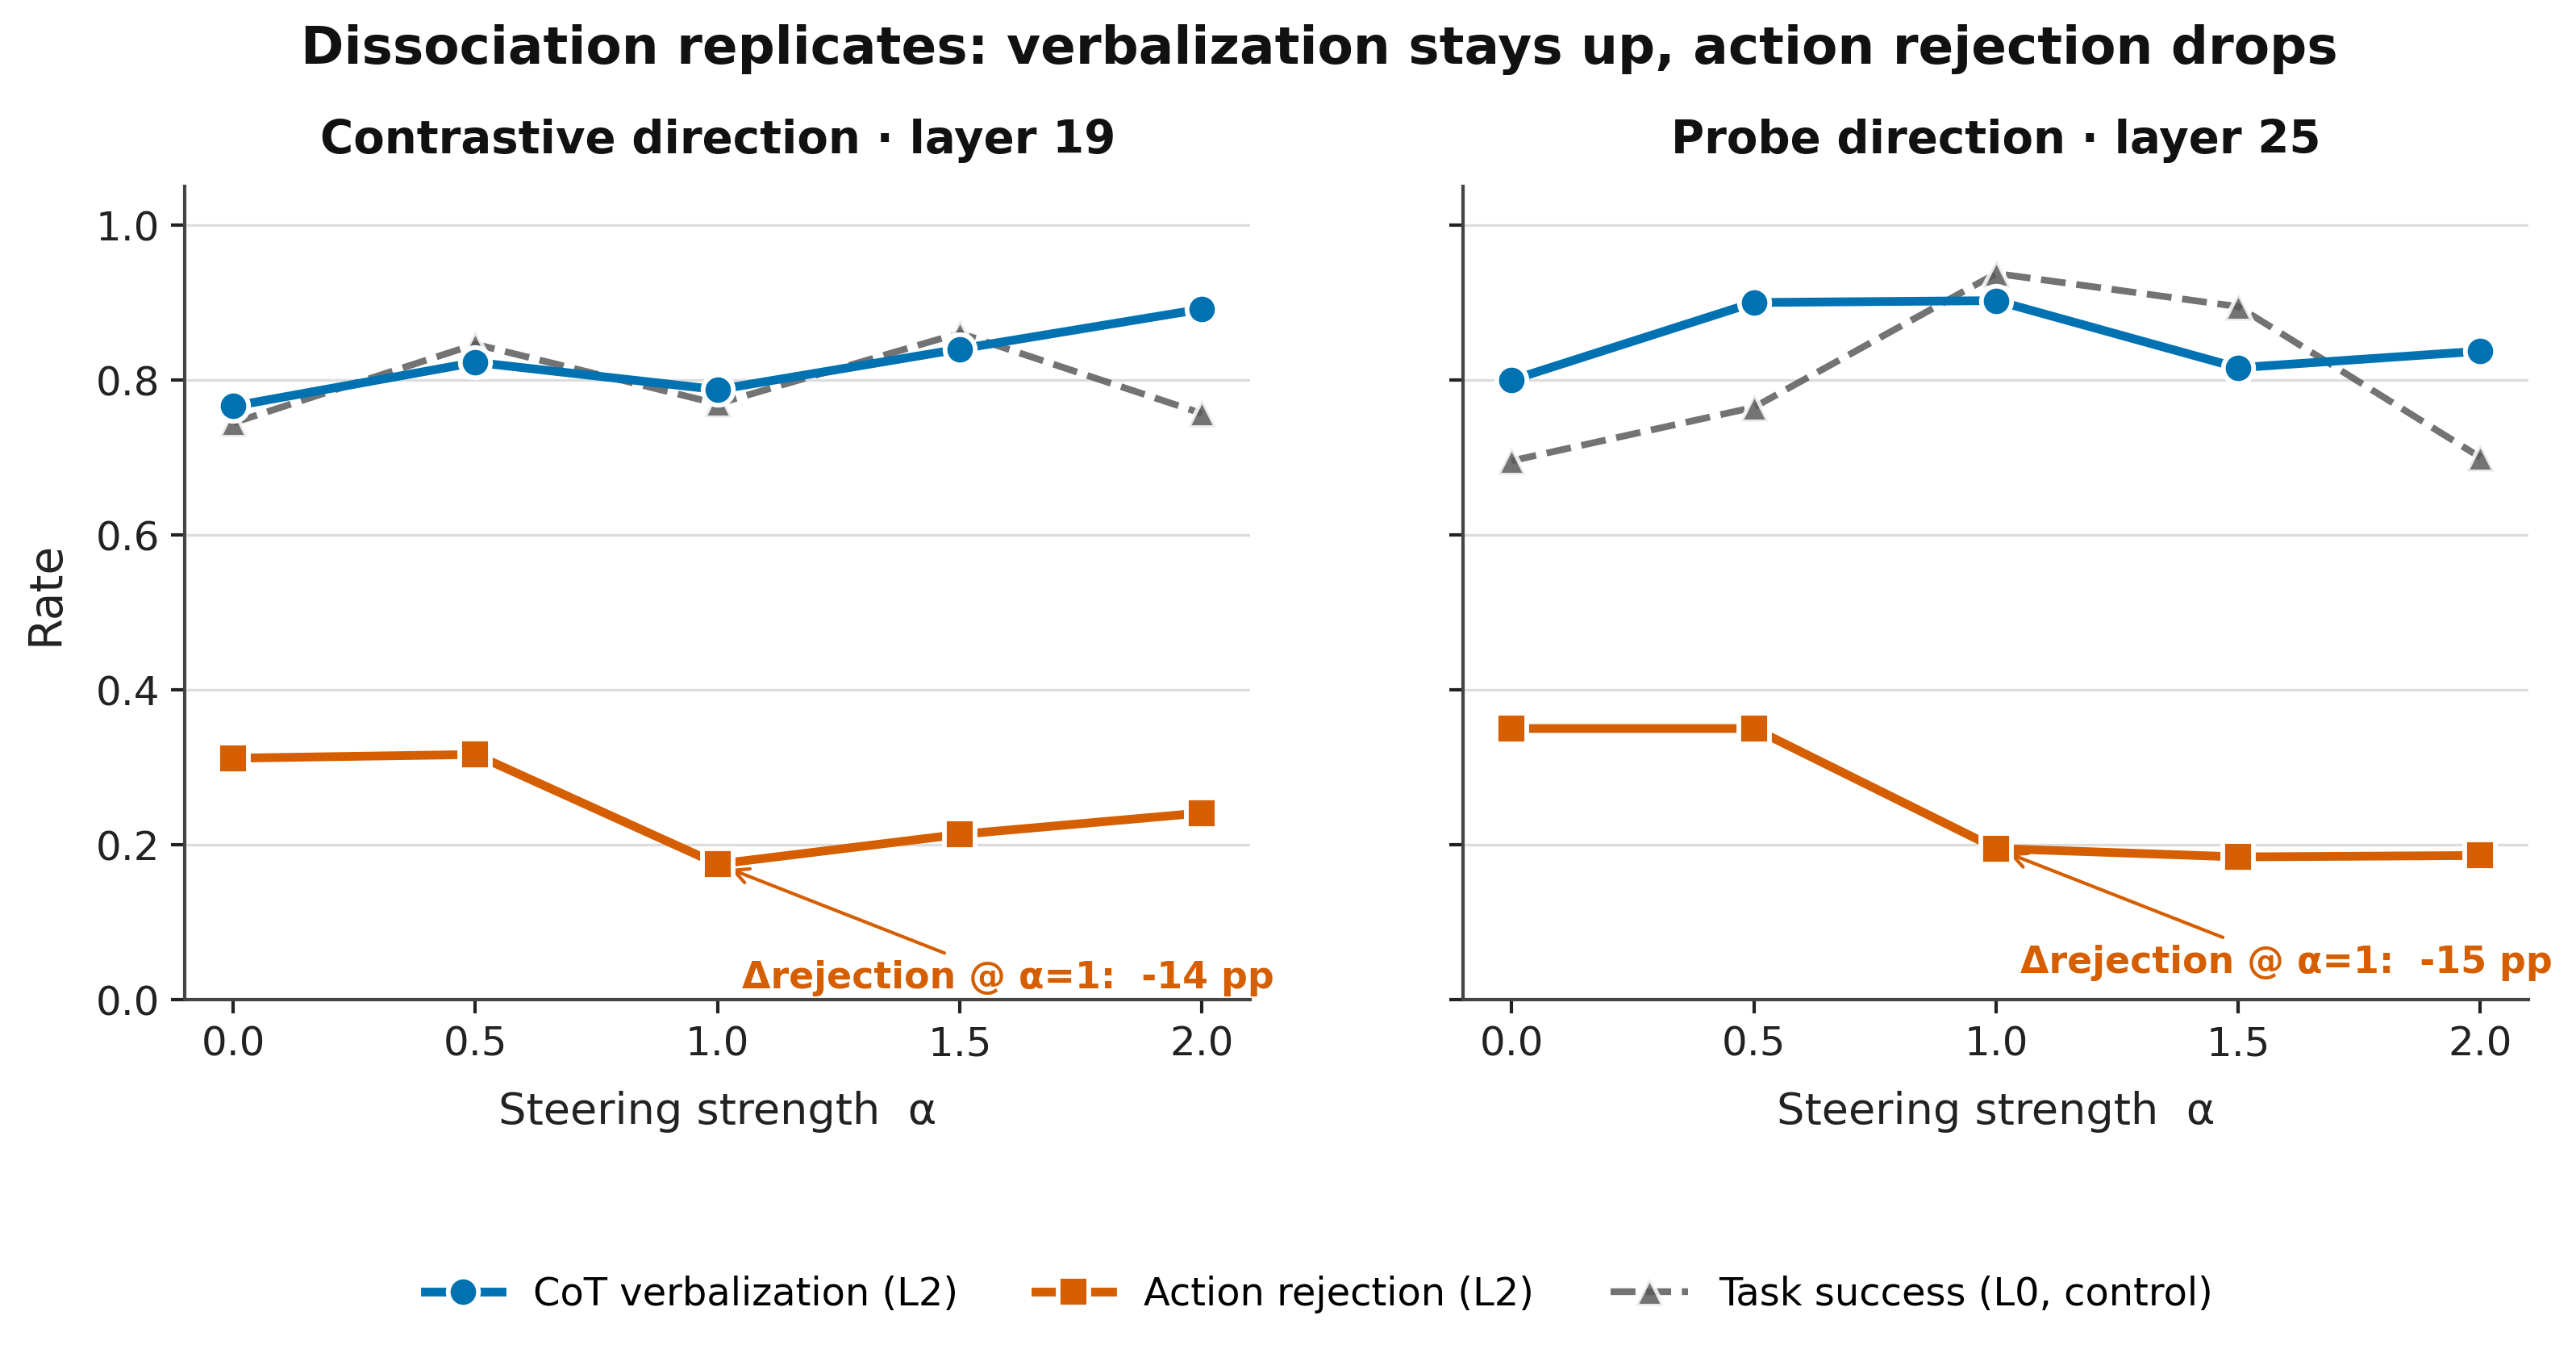
\includegraphics[width=0.92\textwidth]{steering_robustness.png}
\caption{Robustness across direction and layer. The two effects ---
verbalization up, action rejection down --- hold qualitatively across
contrastive vs.\ probe-weights directions and across layer 19 vs.\ layer 25.}
\label{fig:steering-robustness}
\end{figure}

One small but important methodological remark: the original probe-at-L19
sweep at $n \approx 40$ initially showed an apparent +10 percentage-point
verbalization lift at $\alpha = 1$. The high-$n$ rerun in
Table~\ref{tab:steering-headline} did not reproduce that lift at
$\alpha = 1$; the real signal lives at $\alpha \geq 1.5$. The original
result was sampling noise within the GPU non-determinism floor, and the
practical lesson is that small steering effects on agent behavior need at
least 80 trajectories per cell to discriminate signal from instance-level
variance. We report the underpowered run only in the ablation table, where
the larger $\alpha = 4$ effect is well above the noise floor and the
$\alpha = 1$ row should be read as suggestive rather than confirmatory.

\subsection{Deliverables}

The project ships four pieces. A reproducibility artifact, the GitHub
repository, runs end-to-end from a fresh clone (\texttt{pip install -r
requirements.txt} followed by \texttt{python scripts/01\_generate\_corpus.py
--n\_trajectories 10} produces ten valid trajectories on a GPU). The
trajectory dataset comprises 1{,}218 valid trajectories across three seeds,
with the catalog and the per-step activation tensors stored alongside. Four
figures --- \texttt{probe\_auc\_by\_layer.png}, \texttt{three\_curve\_plot.png},
\texttt{steering\_curve.png}, and \texttt{steering\_robustness.png} ---
are included in this report. The test suite, 45 passing CPU-only pytest
cases, locks in the structural invariants of the synthetic environment.

\subsection{Team-member contributions}

This project was developed primarily as a solo effort. The author was
responsible for project design, the synthetic environment, the agent loop,
the activation-capture pipeline, probe training, steering experiments, cloud
infrastructure (A100/H100 host setup, artifact-store layout, parallel-seed
scheduling), and write-up. Where the report uses ``we,'' it follows the
plural-of-modesty convention of academic writing.

% Optional template for a multi-author project:
% \begin{tabular}{lp{0.7\textwidth}}
% \toprule
% Member & Contribution \\
% \midrule
% A.~Name & Synthetic environment, perturbation design, free labels, tests. \\
% B.~Name & Agent loop, activation hooks, corpus generation. \\
% C.~Name & Probe training, steering experiments, figures, report. \\
% \bottomrule
% \end{tabular}

% ===============================================================
\section{Key Takeaways and Future Work}
% ===============================================================

The single sentence we would write to summarize this project is that, in a
tool-use setting, an LLM agent's residual stream contains a near-perfect
linear signal of goal-relative inconsistency that neither its chain of
thought nor its action consistently reflects, and the gap between these is
mechanistically structured rather than noise. The supporting story has
three pieces. A controlled synthetic environment, with matched L1/L2
levels and deterministic free labels, made it possible to claim that a probe
direction is goal-relative rather than input-distance --- a claim a Webshop
scrape cannot support. Standard probing and steering tools developed for
chat models transfer cleanly to mid-trajectory residuals on a 7B
function-calling agent, with no architectural change. And the steering
result is more informative than the predictive result alone: the very
direction that drives more saying drives less acting, which means
unfaithfulness is not a single channel waiting to be aligned but at least
two channels that come apart under intervention.

We would qualify those claims with a handful of limitations. We did not
validate transfer to a non-synthetic benchmark; we ran one model only, and
the absolute AUC and steering magnitudes are likely model-specific even if
the qualitative story generalizes. The verbalization label is regex-based,
which the action-rejection label (purely structural) is not; the two labels
agree in direction, but a paraphrase-aware labeler would tighten the
verbalization curve. The permutation control script is in place but not yet
executed; running it would harden the interpretive ceiling on the 0.96 AUC
number. And the practical noise floor for any single $(\alpha,\,\mathrm{run})$
cell at $n \approx 40$ on H100 is about five percentage points, which is
why we treat the high-$n$ sweep as the headline and the ablation table as
qualitative confirmation.

The natural next steps follow from these limitations. Running the
permutation control and adding an attention-pattern figure for layer 19
would localize the feature beyond ``residual stream at the last
tool-message token.'' Replicating the probe protocol on Webshop and on
\texttt{Llama-3.1-8B-Instruct} would test whether the 0.96 AUC and the
verb-up/rej-down dissociation are model-specific. Running the inverse
intervention --- steering with $\alpha < 0$, \emph{away} from L2-likeness
on L2 trajectories, to see whether either CoT or action move toward
greater rejection --- is the experiment we did not have time for; a
preliminary scaffold sits in \texttt{data/steering\_summaries/steering\_neg}.
And finally, the located probe is cheap enough to deploy: a single
logistic regressor at one mid-network layer, run alongside the agent loop,
would be an independent ``did this tool output disagree with the goal?''
signal whose calibration could be reported every time the CoT and the
action disagree. That is the version of this work that most directly
serves the original safety motivation, and it is a one-week extension
rather than a one-quarter one.

% ===============================================================
\bibliographystyle{plainnat}
\begin{thebibliography}{10}

\bibitem[Alain and Bengio(2016)]{alain2016probes}
G.~Alain and Y.~Bengio.
\newblock Understanding intermediate layers using linear classifier probes.
\newblock {\em arXiv preprint arXiv:1610.01644}, 2016.

\bibitem[Belinkov(2022)]{belinkov2022probing}
Y.~Belinkov.
\newblock Probing classifiers: Promises, shortcomings, and advances.
\newblock {\em Computational Linguistics}, 48(1):207--219, 2022.

\bibitem[Chen et~al.(2025)]{chen2025faith}
Y.~Chen et~al.
\newblock Reasoning models don't always say what they think.
\newblock Anthropic Technical Report, 2025.

\bibitem[Li et~al.(2023)]{li2023othello}
K.~Li, A.~K. Hopkins, D.~Bau, F.~Vi{\'e}gas, H.~Pfister, and M.~Wattenberg.
\newblock Emergent world representations: Exploring a sequence model
  trained on a synthetic task.
\newblock In {\em ICLR}, 2023.

\bibitem[Panickssery et~al.(2024)]{panickssery2024caa}
N.~Panickssery, N.~Gabrieli, J.~Schulz, M.~Tong, E.~Hubinger, and A.~Turner.
\newblock Steering Llama 2 via contrastive activation addition.
\newblock {\em arXiv preprint arXiv:2312.06681}, 2024.

\bibitem[Qin et~al.(2024)]{qin2024toolllm}
Y.~Qin et~al.
\newblock ToolLLM: Facilitating large language models to master 16000+
  real-world APIs.
\newblock In {\em ICLR}, 2024.

\bibitem[Qwen Team(2024)]{qwen25}
Qwen Team.
\newblock Qwen2.5: A party of foundation models.
\newblock Technical report, Alibaba Group, 2024.

\bibitem[Shridhar et~al.(2021)]{shridhar2021alfworld}
M.~Shridhar, X.~Yuan, M.-A. C{\^o}t{\'e}, Y.~Bisk, A.~Trischler, and
  M.~Hausknecht.
\newblock {ALFWorld}: Aligning text and embodied environments for
  interactive learning.
\newblock In {\em ICLR}, 2021.

\bibitem[Turner et~al.(2023)]{turner2023actadd}
A.~M. Turner, L.~Thiergart, D.~Udell, G.~Leech, U.~Mini, and M.~MacDiarmid.
\newblock Activation addition: Steering language models without
  optimization.
\newblock {\em arXiv preprint arXiv:2308.10248}, 2023.

\bibitem[Yao et~al.(2022)]{yao2022webshop}
S.~Yao, H.~Chen, J.~Yang, and K.~Narasimhan.
\newblock {WebShop}: Towards scalable real-world web interaction with
  grounded language agents.
\newblock In {\em NeurIPS}, 2022.

\end{thebibliography}

\end{document}
